\section{Related Works}
\begin{frame}{Related Works}
    \begin{minipage}[c]{0.65\textwidth}
        \begin{itemize}
            \item EEG MI Classifier
            \item Dataset Augmentation
            \item User Game Feel and Experience
            \item EEG MI Uses in Real Case-Scenarios
        \end{itemize}
    \end{minipage}
    \begin{minipage}[c]{0.33\textwidth}
        \vspace*{-.5cm}
        \hspace*{-.7cm}
        \begin{tikzpicture}
            \node (page1) [yshift=4.5cm, xshift=-.5cm, rotate=30] {
                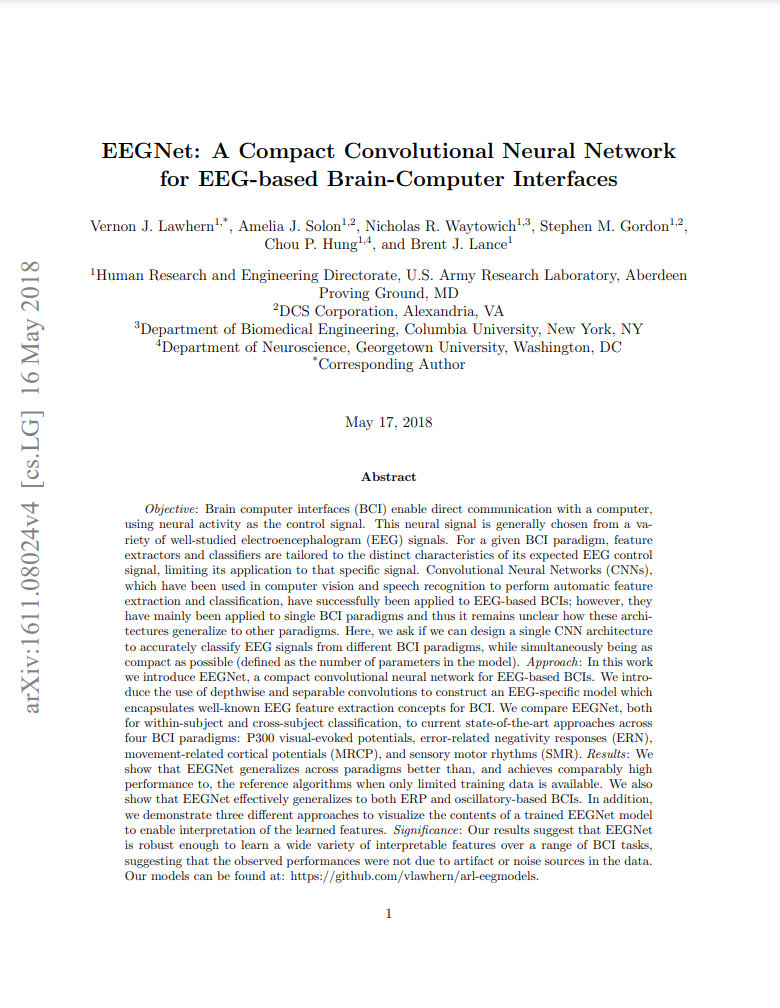
\includegraphics[width=0.4\textwidth]{figures/literature/classifier/EEGNet_paper}
            };
            \node (page2) [yshift=4.5cm, xshift=.5cm, rotate=-30] {
                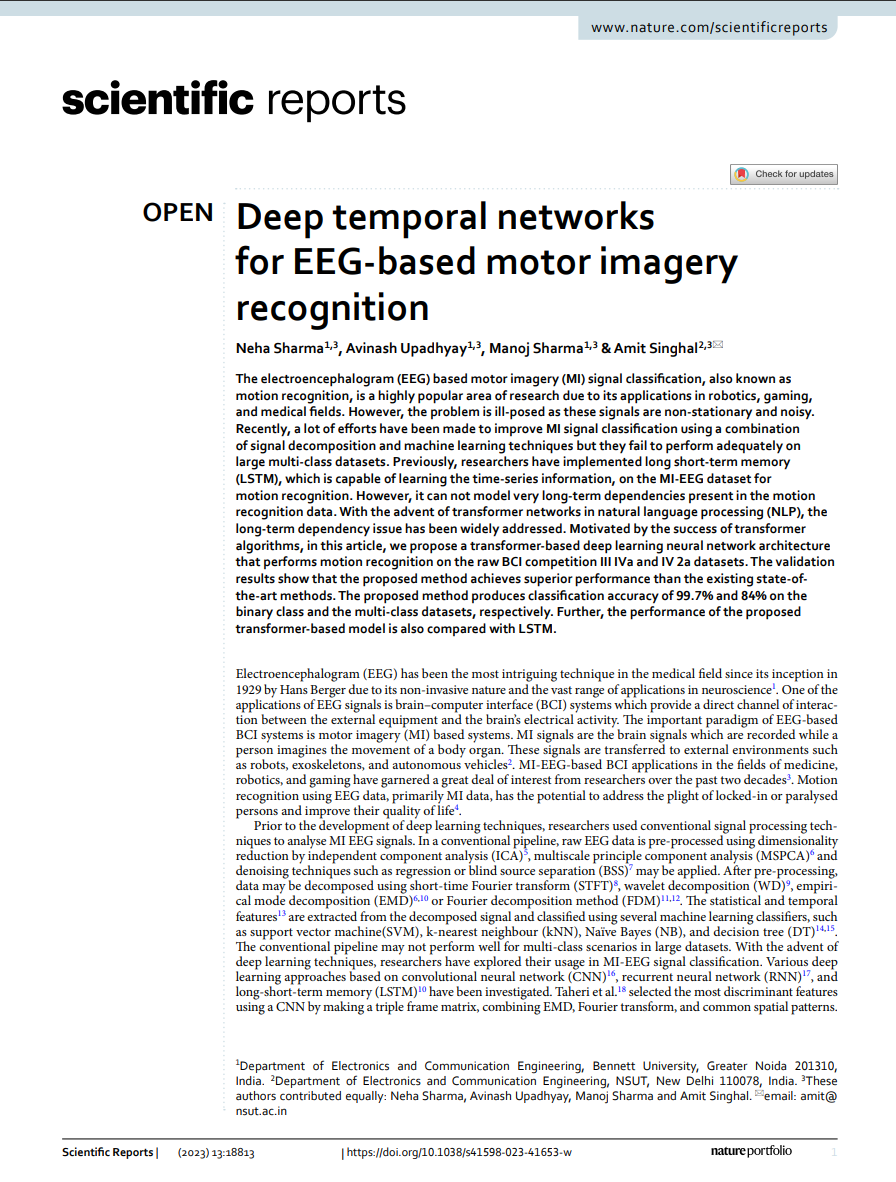
\includegraphics[width=0.4\textwidth]{figures/literature/classifier/LSTM_Transformer_paper}
            };
            %
            \node (page3) [yshift=3cm, xshift=-.5cm, rotate=30] {
                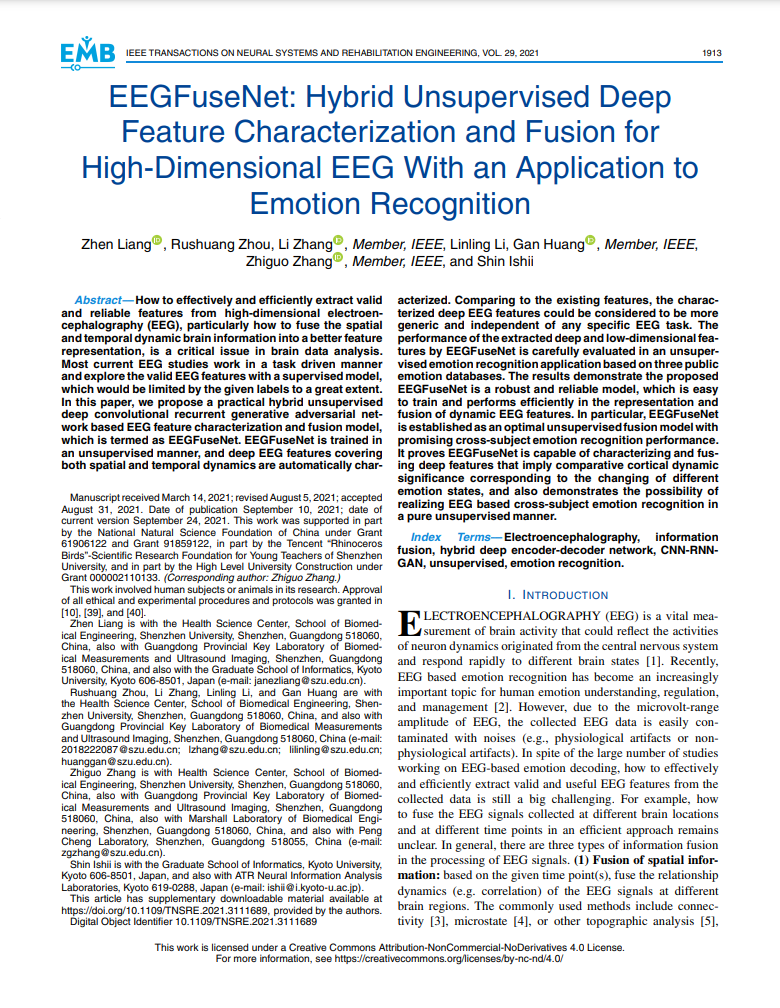
\includegraphics[width=0.4\textwidth]{figures/literature/augmentation/EEGFuseNet_paper}
            };
            \node (page4) [yshift=3cm, xshift=.5cm, rotate=-30] {
                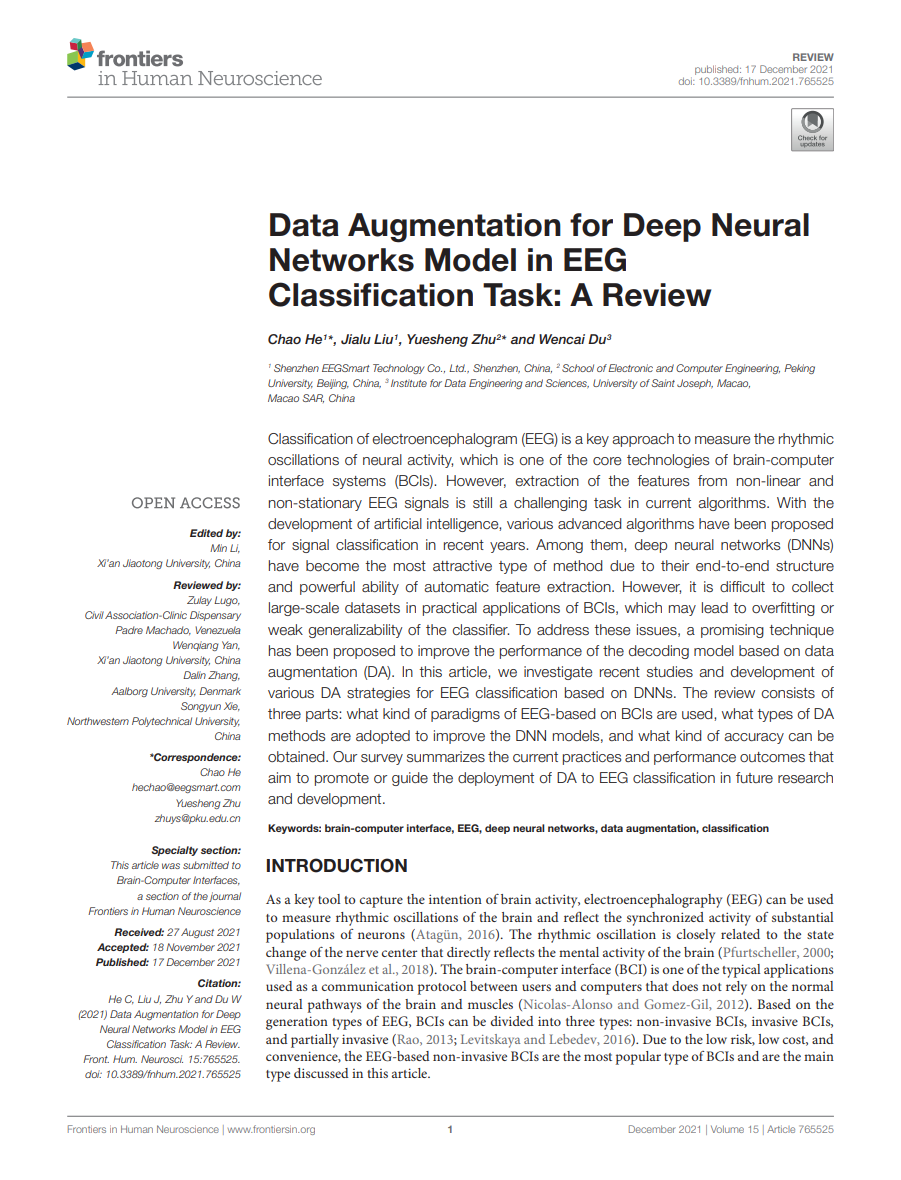
\includegraphics[width=0.4\textwidth]{figures/literature/augmentation/NoiseInjection_paper}
            };
            %
            \node (page5) [yshift=1.5cm, xshift=-.5cm, rotate=30] {
                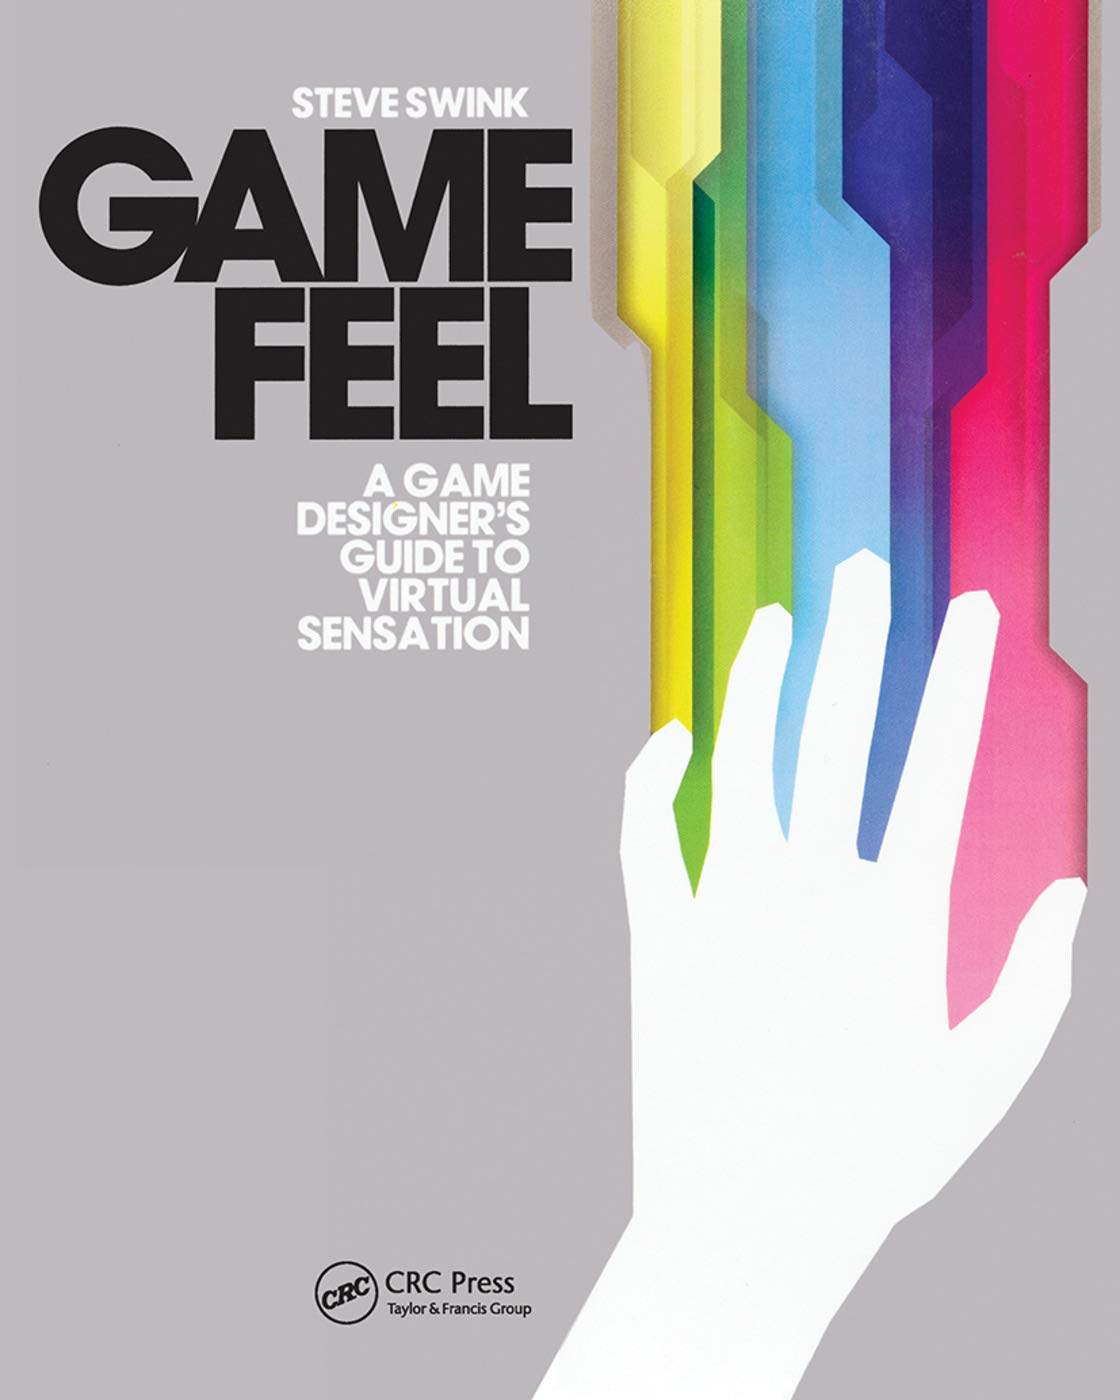
\includegraphics[width=0.4\textwidth]{figures/literature/gamefeel/GameFeel_book}
            };
            \node (page6) [yshift=1.5cm, xshift=.5cm, rotate=-30] {
                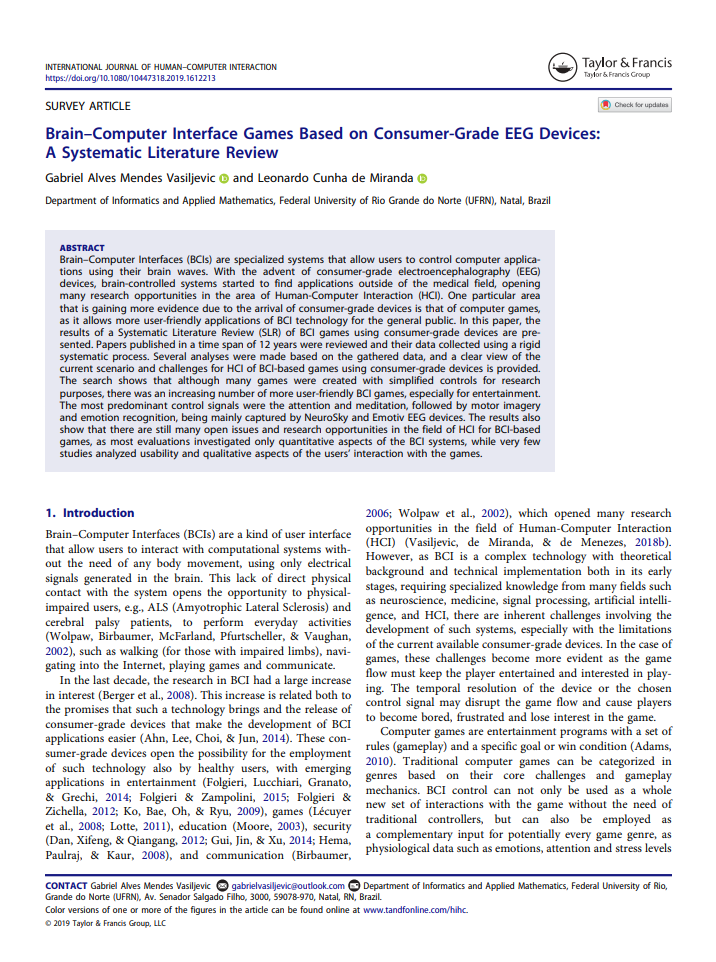
\includegraphics[width=0.4\textwidth]{figures/literature/gamefeel/BCI_Game_paper}
            };
            %
            
            \node (page9) [yshift=0cm, xshift=-1.5cm, rotate=30] {
                
\includegraphics[width=0.4\textwidth]{figures/literature/realcase/WheelchairControl_paper}
            };
            \node (page11) [yshift=0cm, xshift=1.5cm, rotate=-30] {
                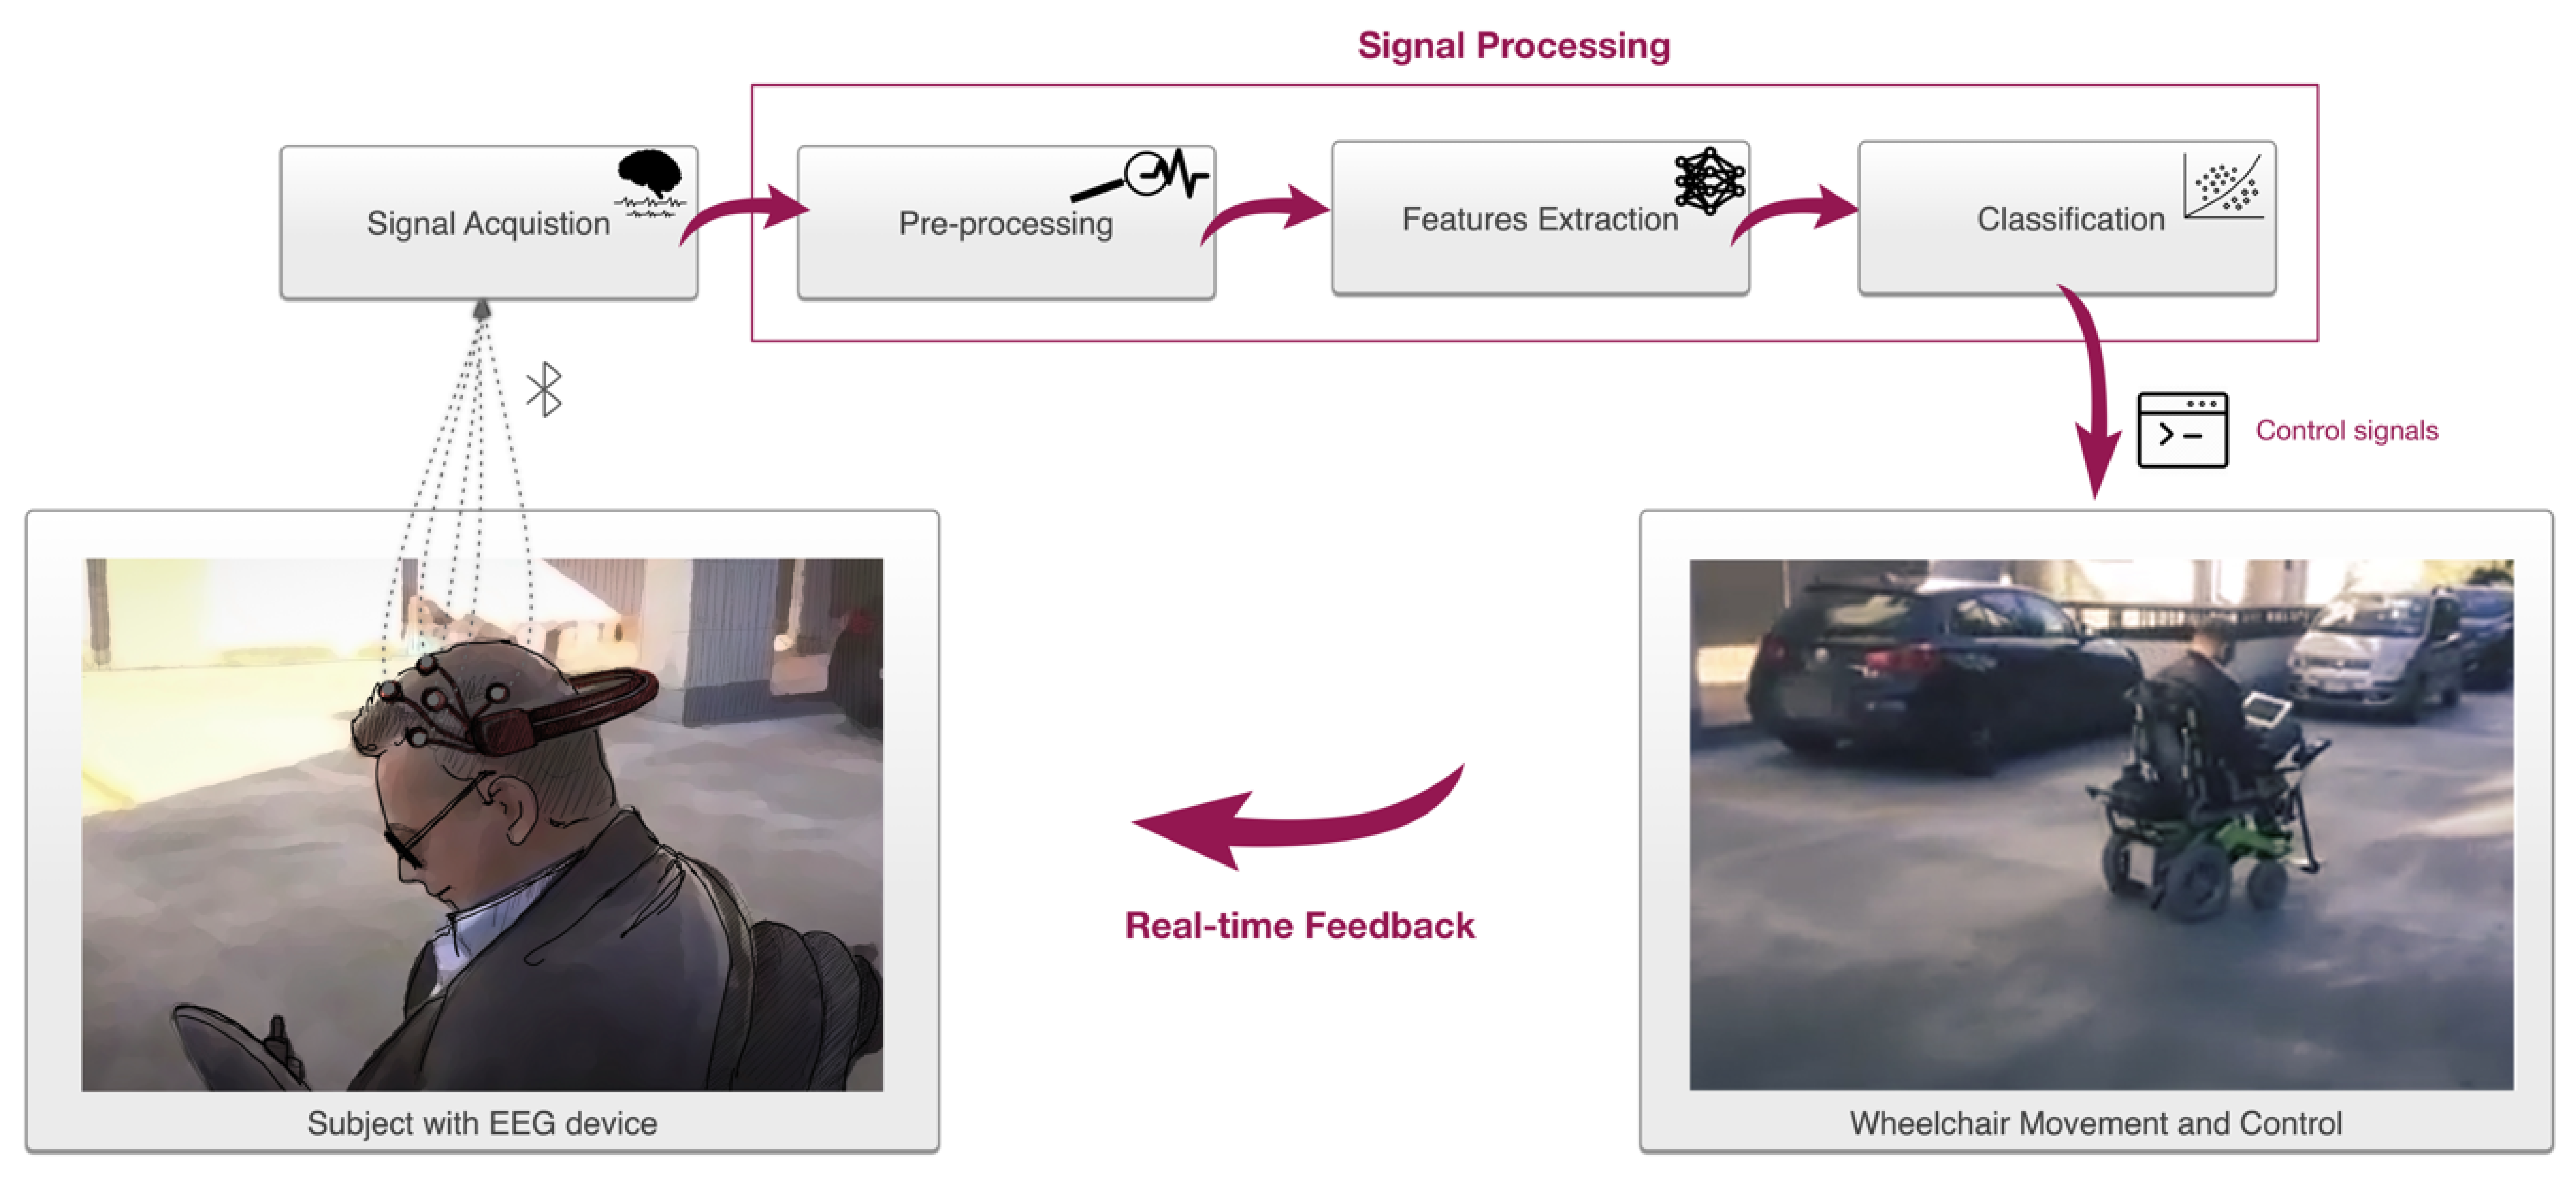
\includegraphics[width=0.4\textwidth]{figures/literature/realcase/wheelchair_control}
            };
            \node (page7) [yshift=0cm, xshift=-.5cm, rotate=30] {
                
\includegraphics[width=0.4\textwidth]{figures/literature/realcase/StrokeRehabilitation_paper}
            };
            \node (page8) [yshift=0cm, xshift=.5cm, rotate=-30] {
                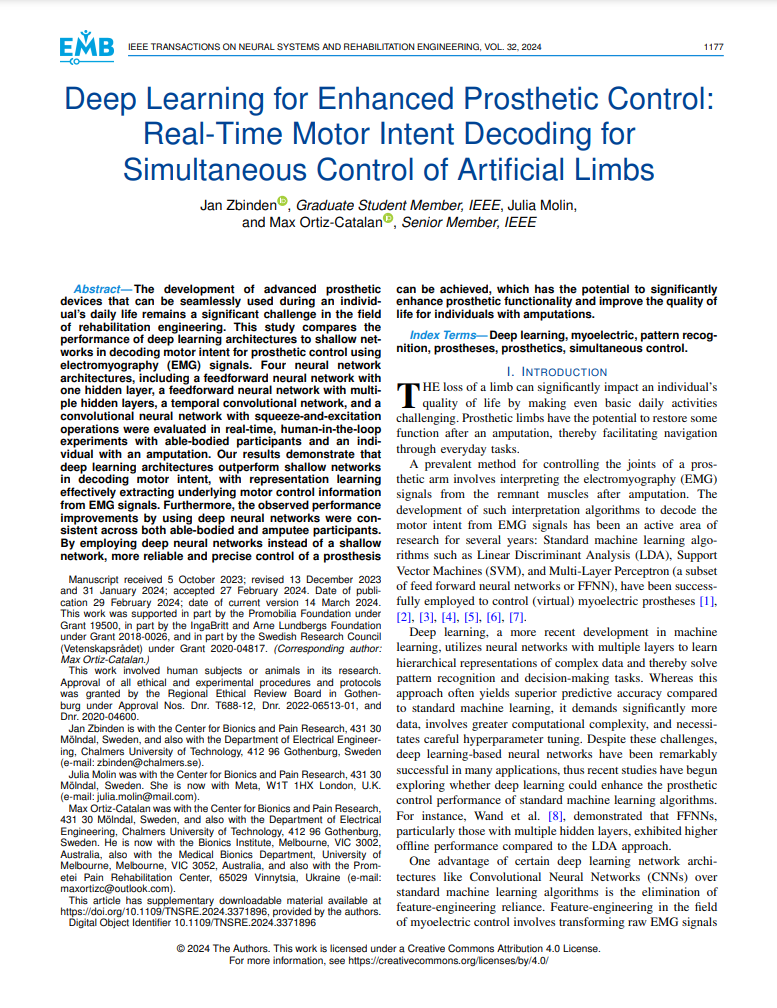
\includegraphics[width=0.4\textwidth]{figures/literature/realcase/ProsthesisControl_paper}
            };
            \node (page10) [yshift=0cm, xshift=0cm, rotate=0] {
                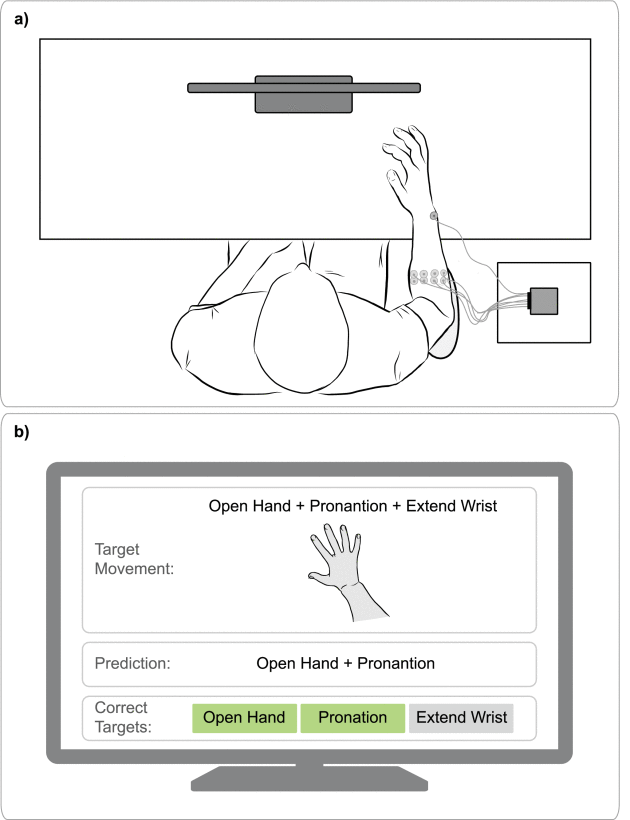
\includegraphics[width=0.4\textwidth]{figures/literature/realcase/limb_control}
            };
        \end{tikzpicture}
    \end{minipage}
\end{frame}

% \begin{frame}{Related Works~\textemdash{}~EEG MI Classifier}
%     \begin{minipage}[c]{0.65\textwidth}
%         \begin{itemize}
%             \item CNN-based approach
%             \item RNN-based approach
%             \item Transformer-based approach
%             \item Machine Learning-based approach
%         \end{itemize}
%     \end{minipage}
%     \begin{minipage}[c]{0.33\textwidth}
%         \vspace*{-.5cm}
%         \hspace*{-.7cm}
%         \begin{tikzpicture}
%             \node (page1) [xshift=-.7cm, rotate=30] {
%                 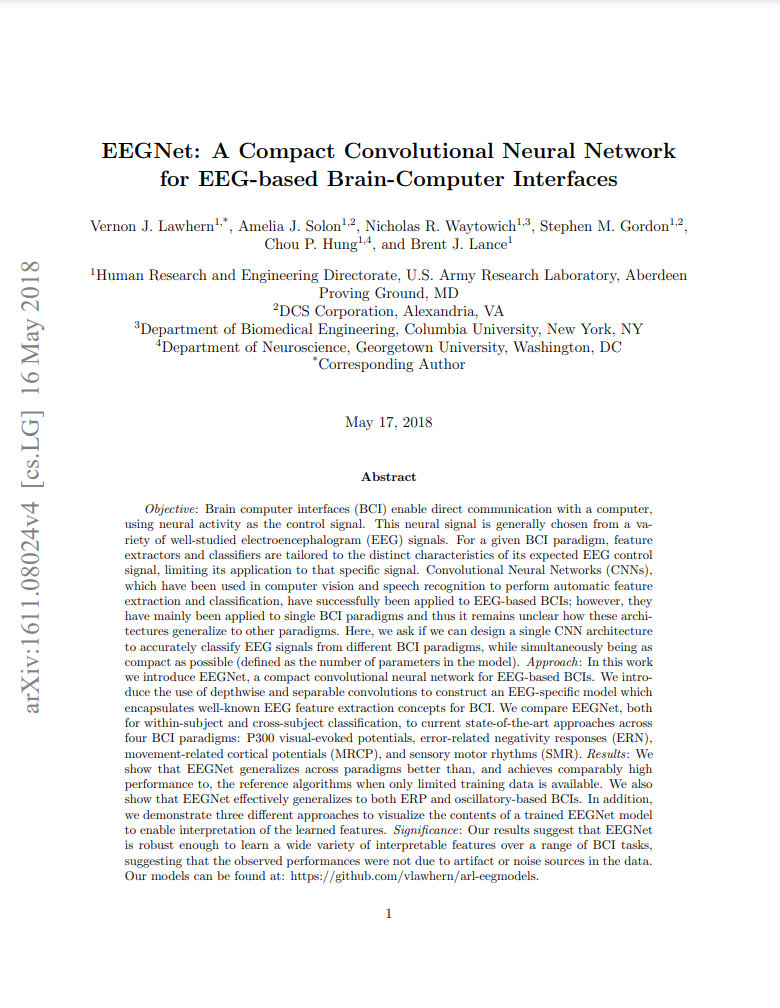
\includegraphics[width=0.6\textwidth]{figures/literature/classifier/EEGNet_paper}
%             };
%             \node (page2) [xshift=.7cm, rotate=-30] {
%                 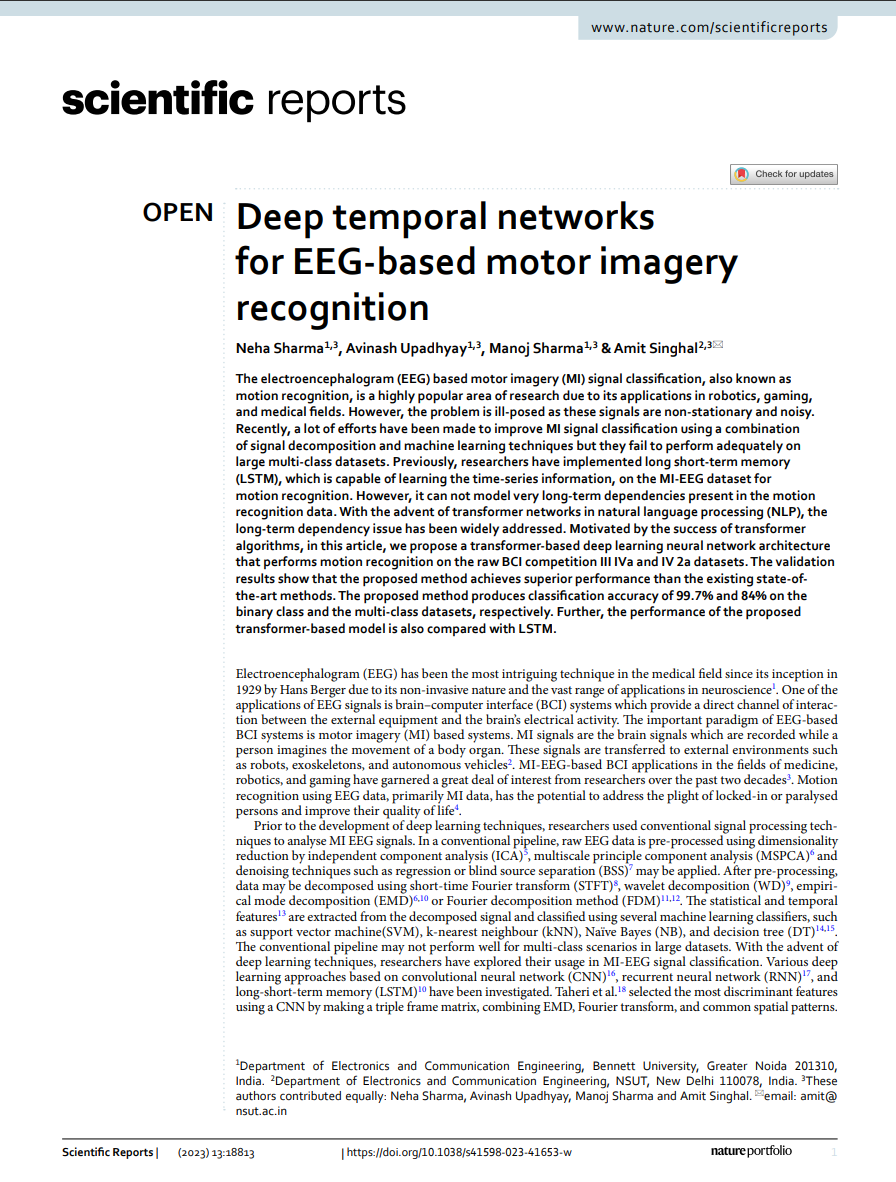
\includegraphics[width=0.6\textwidth]{figures/literature/classifier/LSTM_Transformer_paper}
%             };
%         \end{tikzpicture}
%     \end{minipage}
% \end{frame}
% \begin{frame}{Related Works~\textemdash{}~Dataset Augmentation}
%     \begin{minipage}[c]{0.65\textwidth}
%         \begin{itemize}
%             \item Generative Adversarial Networks (GANs)
%             \item Noise Injection
%             \item Random Sampling
%         \end{itemize}
%     \end{minipage}
%     \begin{minipage}[c]{0.33\textwidth}
%         \vspace*{-.5cm}
%         \hspace*{-.7cm}
%         \begin{tikzpicture}
%             \node (page3) [xshift=-.7cm, rotate=30] {
%                 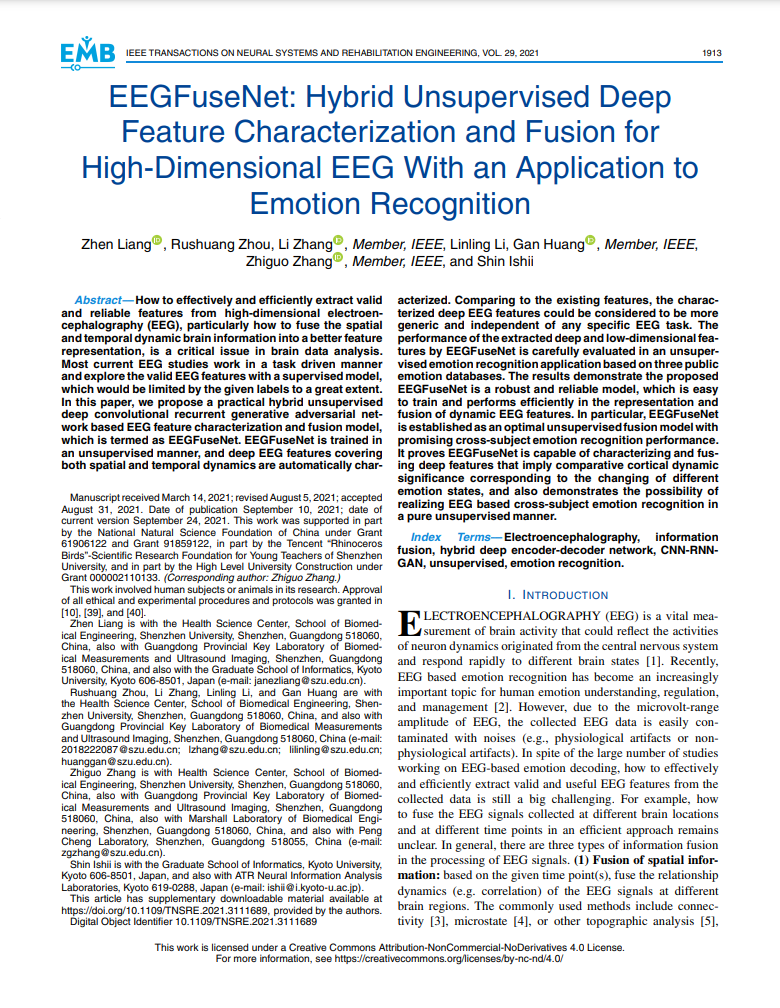
\includegraphics[width=0.6\textwidth]{figures/literature/augmentation/EEGFuseNet_paper}
%             };
%             \node (page4) [xshift=.7cm, rotate=-30] {
%                 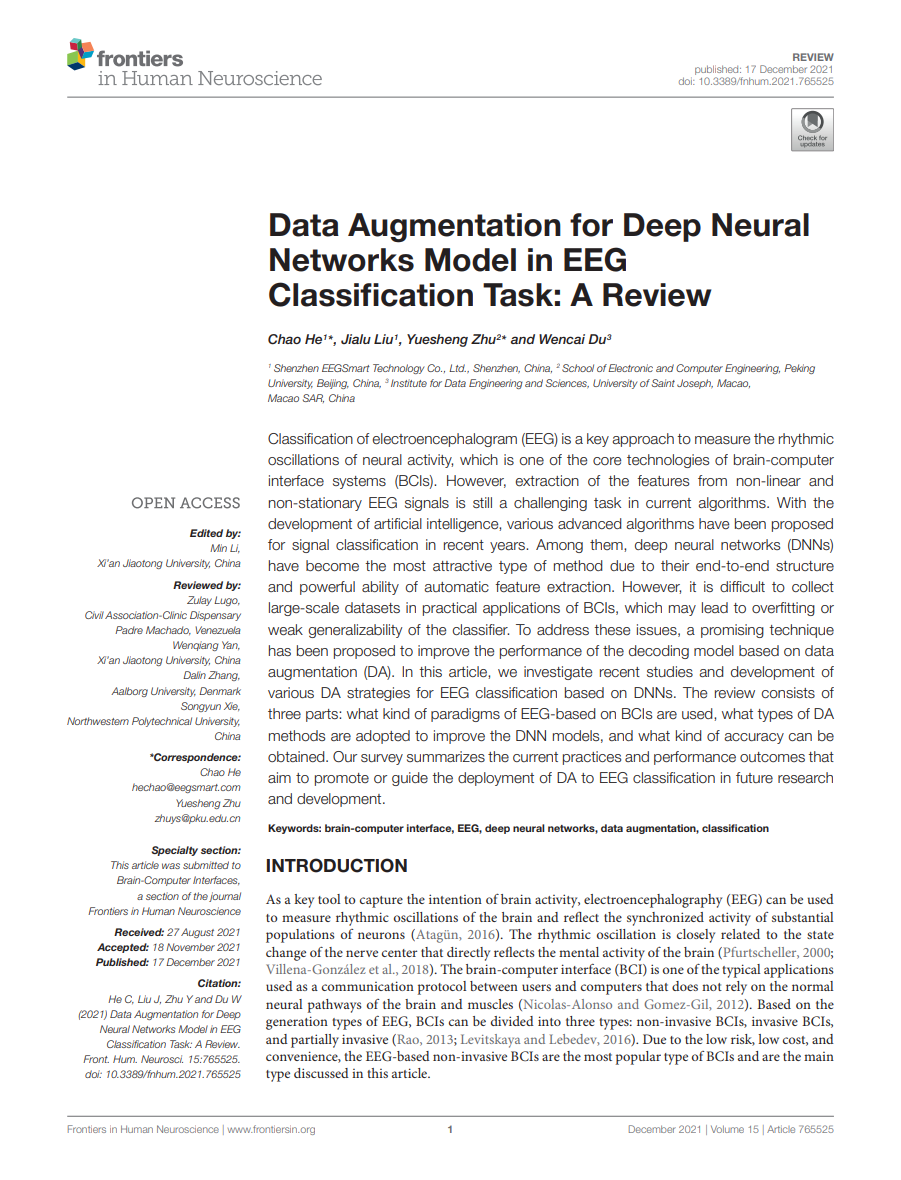
\includegraphics[width=0.6\textwidth]{figures/literature/augmentation/NoiseInjection_paper}
%             };
%         \end{tikzpicture}
%     \end{minipage}
% \end{frame}
% \begin{frame}{Related Works~\textemdash{}~User Game Feel and Experience}
%     \begin{minipage}[c]{0.65\textwidth}
%         \begin{itemize}
%             \item Engagement
%             \item Flow
%             \item Immersion
%             \item Presence
%         \end{itemize}
%     \end{minipage}
%     \begin{minipage}[c]{0.33\textwidth}
%         \vspace*{-.5cm}
%         \hspace*{-.7cm}
%         \begin{tikzpicture}
%             \node (page5) [xshift=-.7cm, rotate=30] {
%                 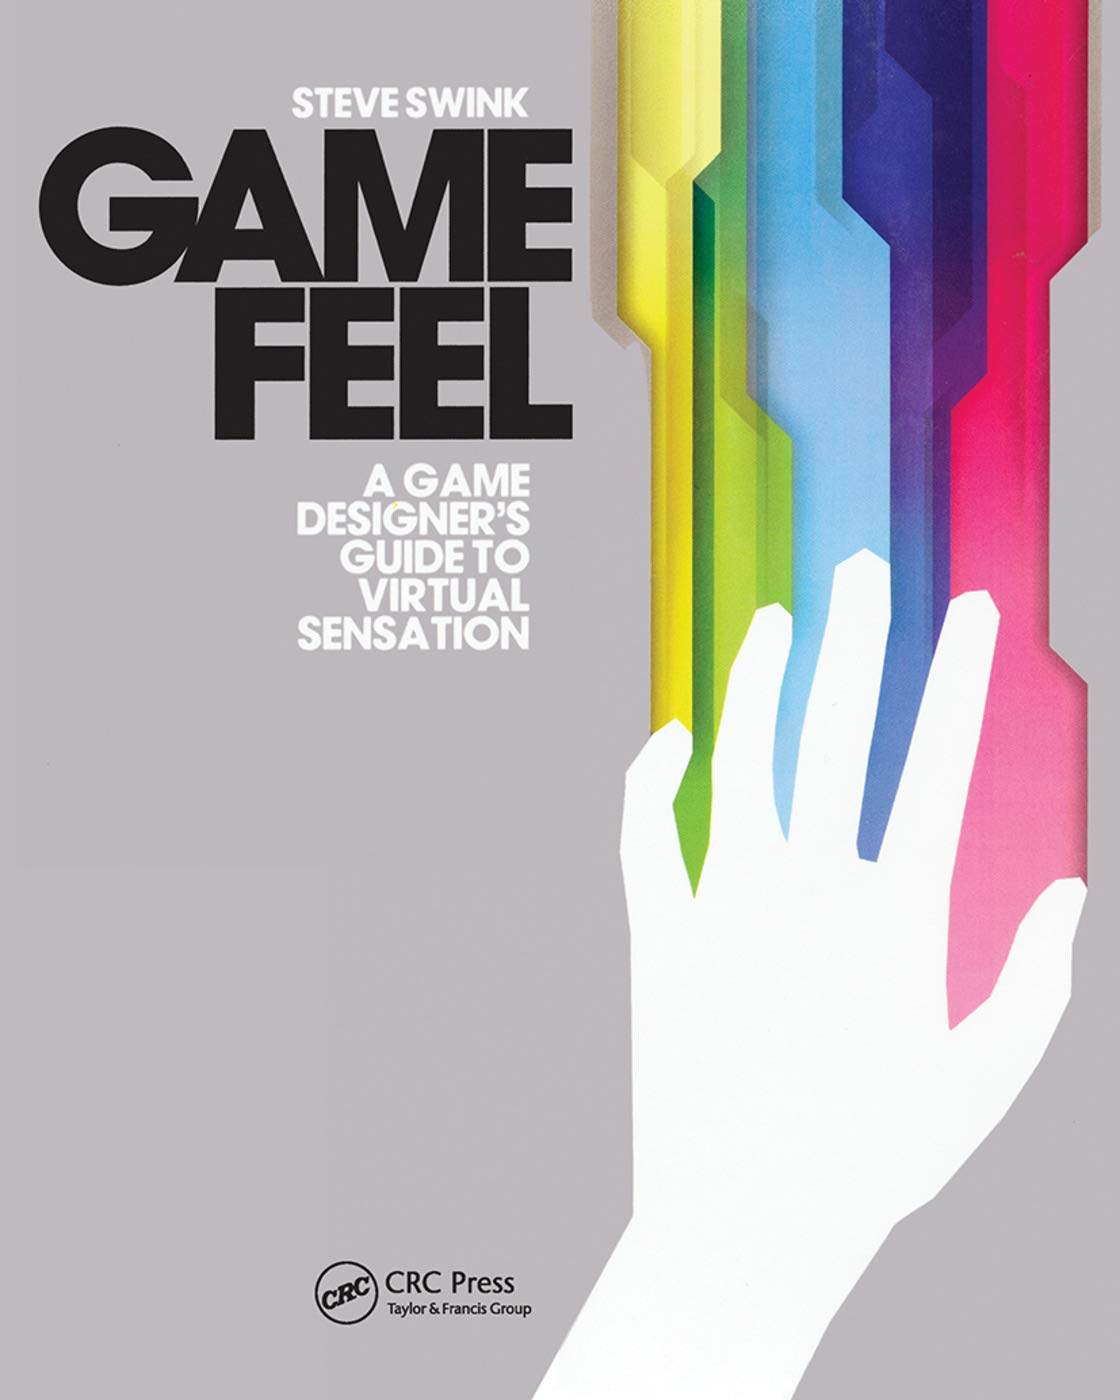
\includegraphics[width=0.6\textwidth]{figures/literature/gamefeel/GameFeel_book}
%             };
%             \node (page6) [xshift=.7cm, rotate=-30] {
%                 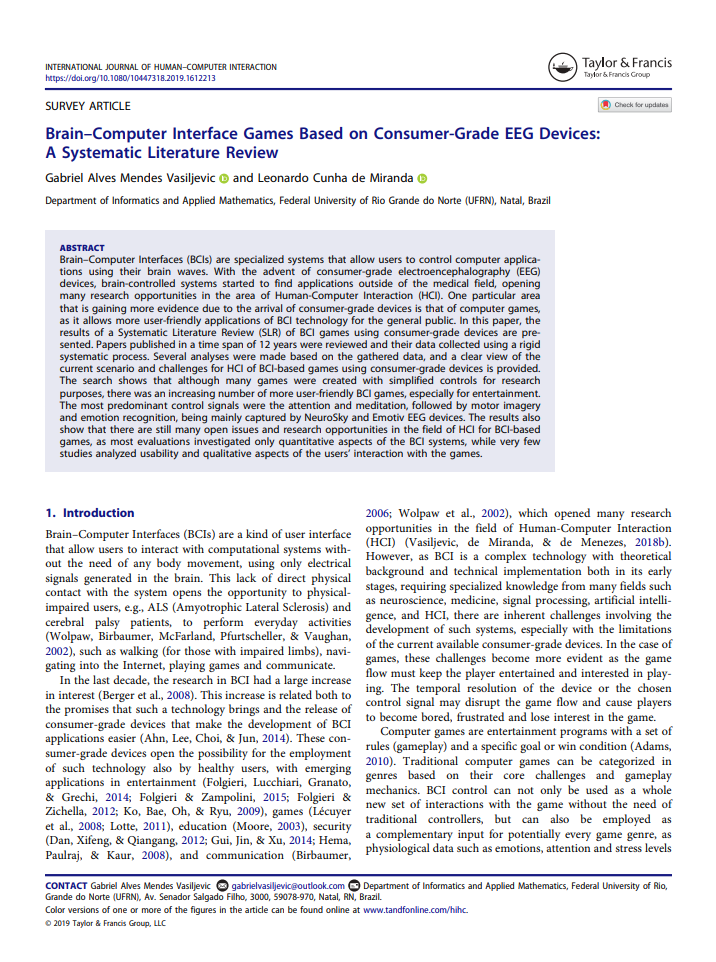
\includegraphics[width=0.6\textwidth]{figures/literature/gamefeel/BCI_Game_paper}
%             };
%         \end{tikzpicture}
%     \end{minipage}
% \end{frame}
% \begin{frame}{Related Works~\textemdash{}~EEG MI Uses in Real Case-Scenarios}
%     \begin{minipage}[c]{0.65\textwidth}
%         \begin{itemize}
%             \item Post-Stroke Rehabilitation
%             \item Prosthesis Control
%             \item Wheelchair Control
%         \end{itemize}
%     \end{minipage}
%     \begin{minipage}[c]{0.33\textwidth}
%         \vspace*{-.5cm}
%         \hspace*{-.7cm}
%         \begin{tikzpicture}
%             \node (page8) [yshift=1cm, xshift=-.75cm, rotate=30] {
%                 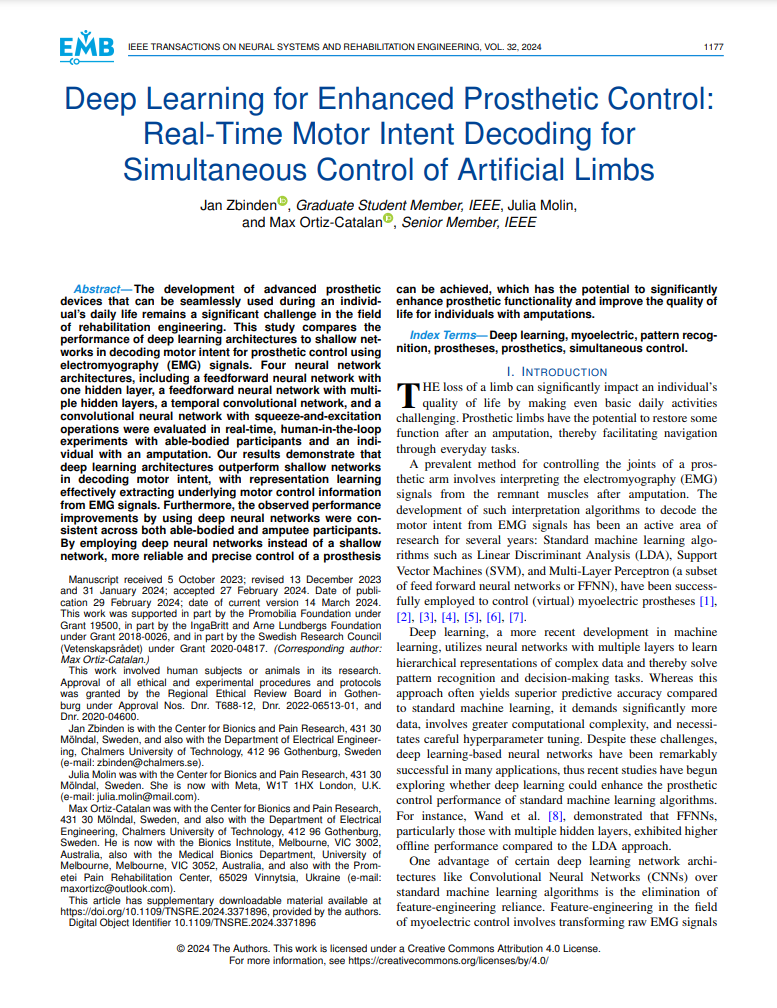
\includegraphics[width=0.65\textwidth]{figures/literature/realcase/ProsthesisControl_paper}
%             };
%             \node (page7) [yshift=1cm, xshift=.75cm, rotate=-30] {
%                 
\includegraphics[width=0.65\textwidth]{figures/literature/realcase/StrokeRehabilitation_paper}
%             };
%             \node (page10) [yshift=0cm, xshift=0cm, rotate=0] {
%                 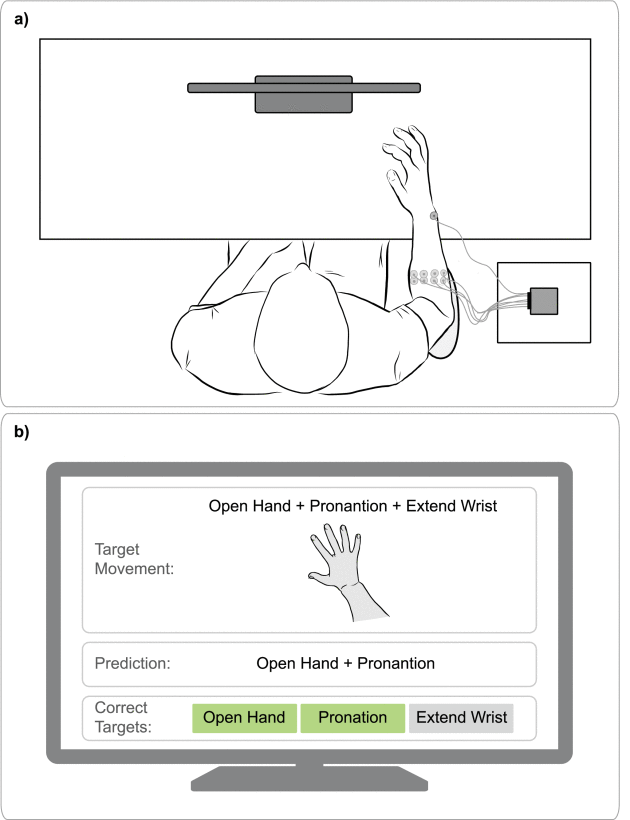
\includegraphics[width=0.65\textwidth]{figures/literature/realcase/limb_control}
%             };
%             \node (page9) [yshift=-1.5cm, xshift=.75cm, rotate=-30] {
%                 
\includegraphics[width=0.65\textwidth]{figures/literature/realcase/WheelchairControl_paper}
%             };
%             \node (page11) [yshift=-1.5cm, xshift=-.75cm, rotate=30] {
%                 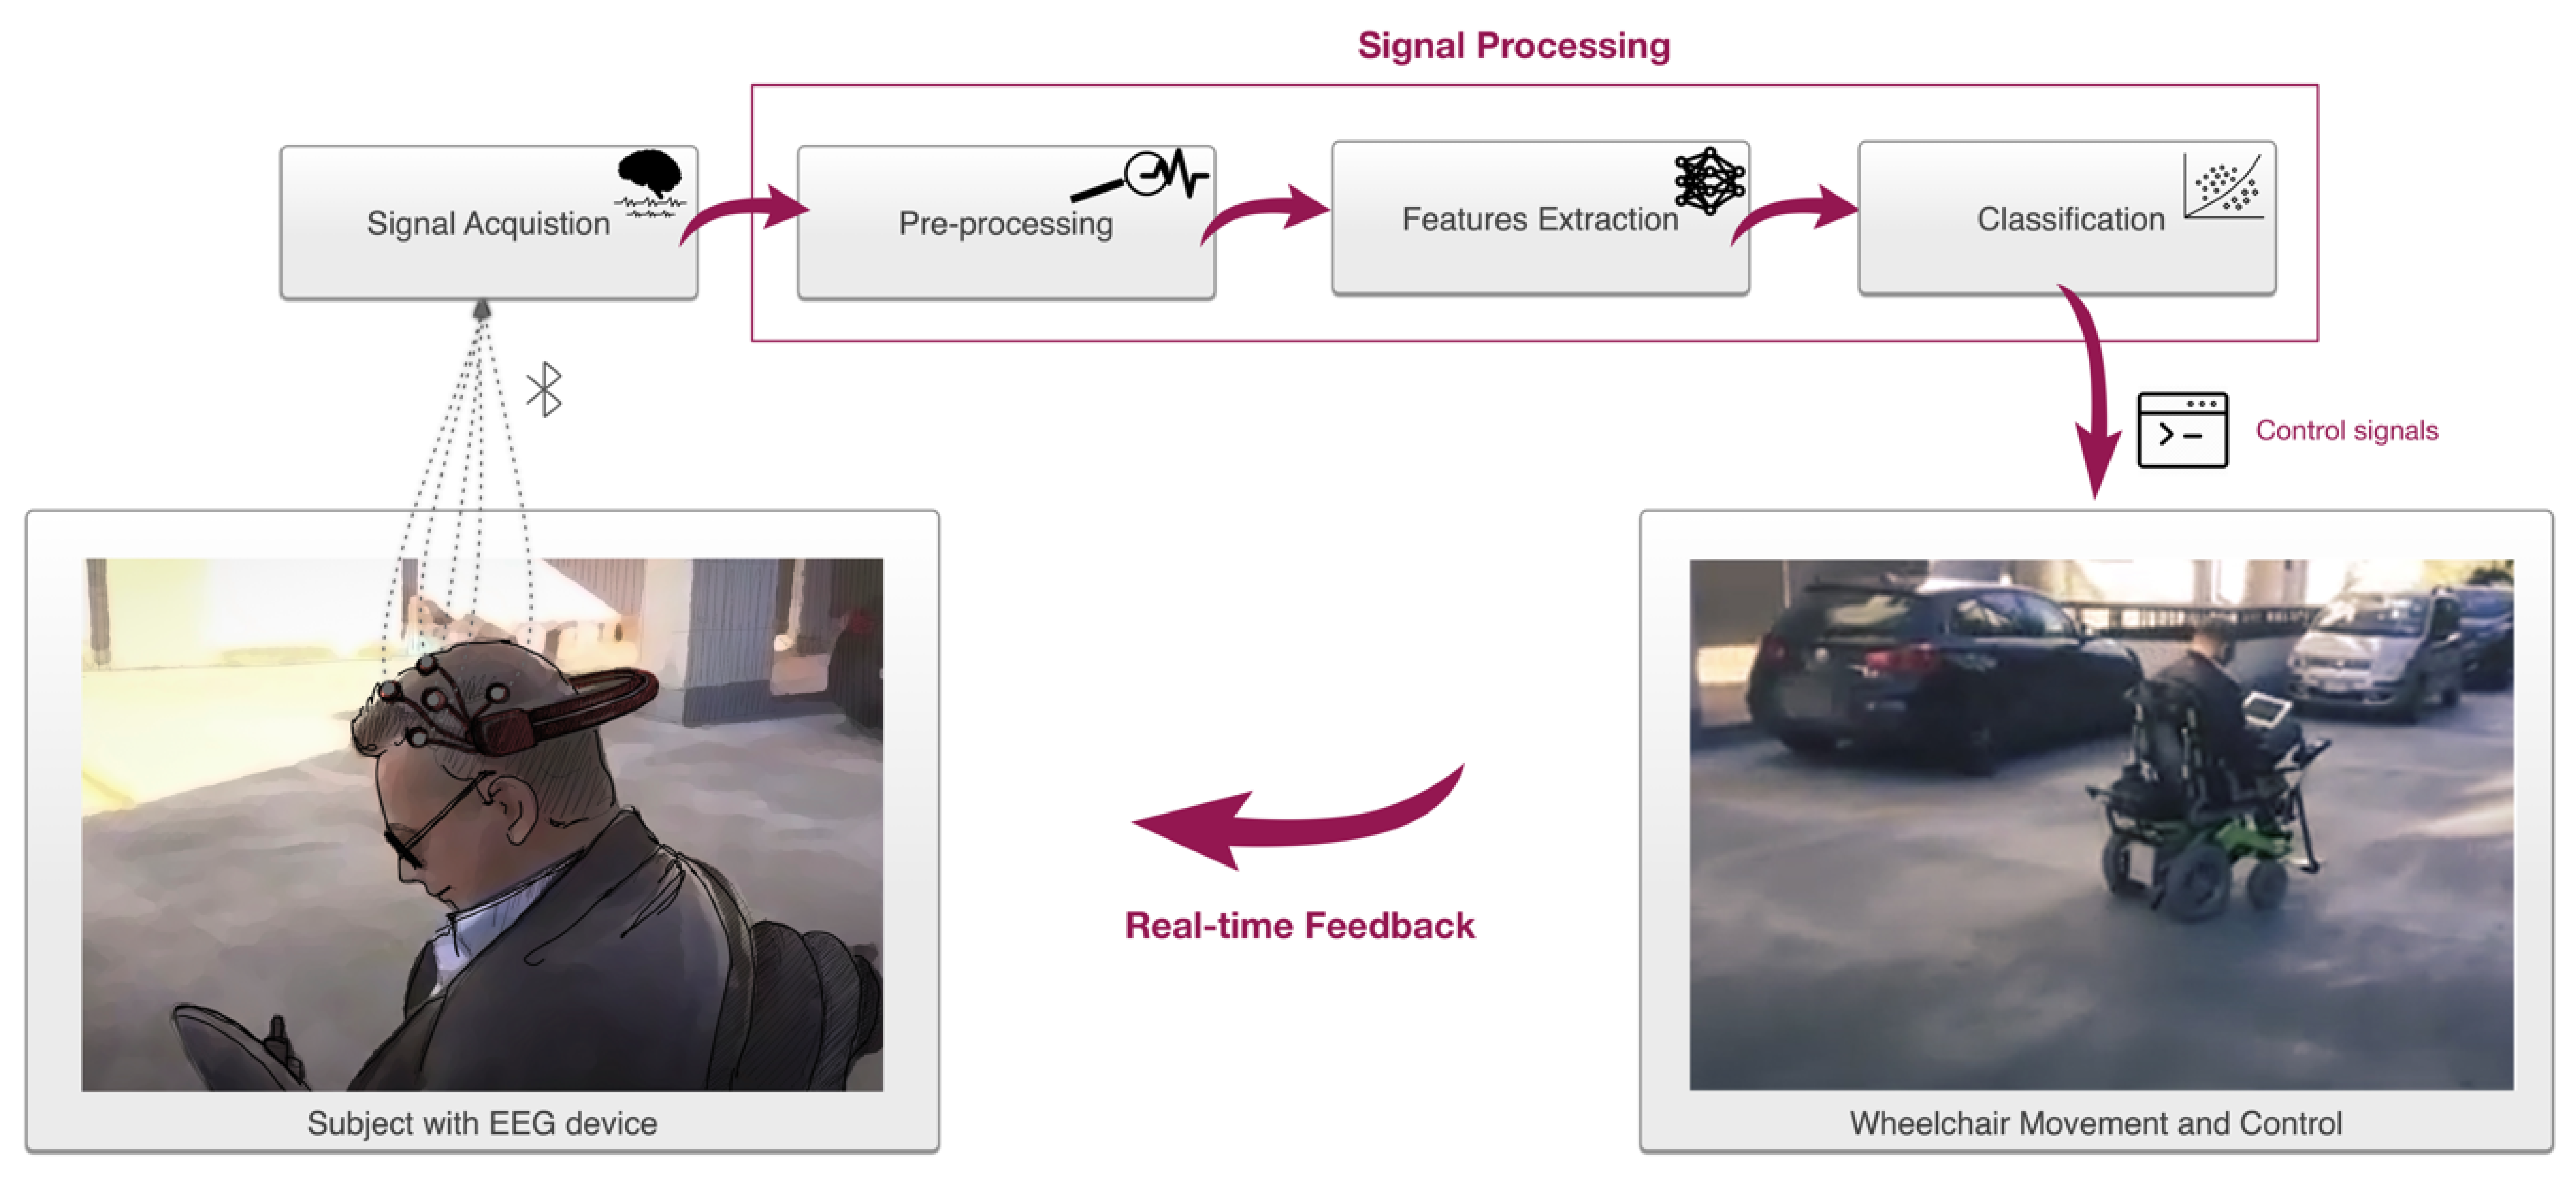
\includegraphics[width=0.65\textwidth]{figures/literature/realcase/wheelchair_control}
%             };
%         \end{tikzpicture}
%     \end{minipage}
% \end{frame}
